\documentclass{article}

\usepackage{arxiv}

\usepackage[utf8]{inputenc} % allow utf-8 input
\usepackage[T1]{fontenc}    % use 8-bit T1 fonts
\usepackage{hyperref}       % hyperlinks
\usepackage{url}            % simple URL typesetting
\usepackage{booktabs}       % professional-quality tables
\usepackage{amsfonts}       % blackboard math symbols
\usepackage{nicefrac}       % compact symbols for 1/2, etc.
\usepackage{microtype}      % microtypography
\usepackage{cleveref}       % smart cross-referencing
\usepackage{graphicx}
\usepackage{natbib}
\usepackage{doi}
\usepackage{caption}
\usepackage{subcaption}
\usepackage{array}

\title{Can depthwise separable convolution make neural style transfer more lightweight? A Comparative Study}

\author{ 
    \href{https://orcid.org/0000-0000-0000-0000}{\includegraphics[scale=0.06]{orcid.pdf}}\hspace{1mm}Shichao Guo \\
	Department of Computer Science\\
	Aarhus University\\
	\texttt{au779770@uni.au.dk} \\
}

\renewcommand{\shorttitle}{Lightweight Neural Style Transfer}

\newcommand{\img}[1]{\includegraphics[width=3cm, height=3cm, keepaspectratio=false]{#1}}

\begin{document}
\maketitle

\begin{abstract}
This project explores how well Depthwise Separable Convolutions can lower the computing cost of Neural Style Transfer. We implemented a baseline Fast Neural Style Transfer network and three progressive lightweight variants. Our experiments on the COCO 2017 dataset demonstrate that replacing standard convolutions with DSCs can reduce the model size by up to 87.62\% and achieve a 1.44x speedup on CPU inference, while maintaining comparable visual quality.
\end{abstract}

\keywords{Neural Style Transfer \and Depthwise Separable Convolutions}

\section{Introduction}
Neural Style Transfer (NST), first introduced by Gatys et al. \citep{gatys2016image}, has become a popular application of deep learning, allowing users to blend the content of one image with the artistic style of another. While the original optimization-based approach was slow, Johnson et al. \citep{johnson2016perceptual} proposed a feed-forward network (Transformer Net) to generate stylized images in real-time. However, these networks often rely on heavy standard convolution layers, making them computationally expensive for real-time applications on mobile or edge devices.

The objective of this study is to determine if Depthwise Separable Convolutions---a technique popularized by MobileNet \citep{howard2017mobilenets} for efficient computing---can be applied to the style transfer domain to create a "lightweight" generator without significantly compromising artistic quality. We conduct a comparative study across three different levels of architectural modification to answer the question: Can we make style transfer lighter without losing the "style"?

\section{Related Work}
\textbf{Neural Style Transfer:} Gatys et al. \citep{gatys2016image} demonstrated that deep features from Convolutional Neural Networks (CNNs) can separate and recombine image content and style. Johnson et al. \citep{johnson2016perceptual} improved upon this by training a feed-forward network to approximate the optimization process, enabling real-time style transfer.

\textbf{Lightweight Convolutional Neural Networks:} To make convolutional neural networks more efficient and lightweight, reducing computational cost is crucial. Howard et al. \citep{howard2017mobilenets} introduced MobileNets, which utilize Depthwise Separable Convolutions (DSC) to factorize a standard convolution into a depthwise spatial convolution and a pointwise ($1\times1$) channel convolution. This factorization significantly reduces both parameters and computation (FLOPs).

Our work bridges these two fields by integrating DSCs into the architecture of Johnson et al., evaluating the trade-offs between efficiency and visual fidelity.

\section{Methods}

\subsection{Dataset and Preprocessing}
We utilized the \textbf{COCO 2017 Validation Set} as our content image source. Due to computational constraints, we used only the Validation Set of COCO 2017, splitting it into training, validation, and test subsets as follows:
\begin{itemize}
    \item \textbf{Training Set:} 4,455 images
    \item \textbf{Validation Set:} 495 images (used for monitoring training progress)
    \item \textbf{Test Set:} 50 images (reserved for final evaluation)
\end{itemize}
All images were resized to $256 \times 256$ pixels, center-cropped, and added with Gaussian noise (See Table \ref{tab:coco_samples}). 

\begin{table}[htbp]
\centering
\setlength{\tabcolsep}{0pt} % 紧密贴合
\renewcommand{\arraystretch}{0} % 去掉行间隙
\begin{tabular}{ *{5}{ >{\centering\arraybackslash}m{3cm} } }
    % 测试图片000000098497
    \img{../history/1_256.jpg} & 
    \img{../history/2_256.jpg} &
    \img{../history/3_256.jpg} &
    \img{../history/4_256.jpg} &
    \img{../history/5_256.jpg} \\
\end{tabular}
\vspace{5pt} 
\caption{Samples of the MS COCO 2017 Set}
\label{tab:coco_samples}
\end{table}

The style reference image used was Vincent van Gogh's \textit{The Starry Night} (See Figure \ref{fig:starry_night}).

\begin{figure}[h]
    \centering
        \centering
        \includegraphics[width=0.4\textwidth]{../history/starry_night.jpg}
    \caption{Style Image (Starry Night) used for Neural Style Transfer}
    \label{fig:starry_night}
\end{figure}


\subsection{Model Architectures}
We created four versions of the model so we could clearly see how the lightweight layers affect performance.

\textbf{Baseline:} A standard Transformer Net consisting of 3 convolution layers (Encoder), 5 Residual Blocks, and 3 Transposed Convolution layers (Decoder), according to Johnson et al. \citep{johnson2016perceptual}.

\textbf{Lightweight Convolution Layer Design:} We built a \textit{LightweightConvLayer} that replaces the usual spatial convolution in the Baseline model. It uses a depthwise convolution with groups equal to $C_{in}$, then a pointwise convolution with a size of $1 \times 1$. 
We added Instance Normalization and a ReLU function between the depthwise layer and the pointwise layer to ensure non-linearity and stable training.

\textbf{The Variants:}
\begin{itemize}
    \item \textbf{Lightweight-v1:} Replaces only the 5 \textbf{Residual Blocks} with lightweight blocks.
    \item \textbf{Lightweight-v2:} Replaces the \textbf{Encoder} (downsampling layers) and \textbf{Residual Blocks}.
    \item \textbf{Lightweight-v3 (Fully Lightweight):} Replaces the \textbf{Encoder}, \textbf{Residual Blocks}, and the \textbf{Decoder} (upsampling layers).
\end{itemize}

\subsection{Training}
The networks were trained to minimize a Perceptual Loss function ($L_{total} = \lambda_c L_{content} + \lambda_s L_{style} + \lambda_{tv} L_{tv}$), computed using a pre-trained VGG-16 network.
The content loss ($L_{content}$) was calculated using the feature maps, while the style loss ($L_{style}$) was computed using Gram matrices. 
The total variation loss ($L_{tv}$) was included to encourage spatial smoothness in the output images.
\begin{itemize}
    \item \textbf{Optimization:} Adam optimizer ($lr=1e-3$) with \texttt{ReduceLROnPlateau} scheduler.
    \item \textbf{Training Duration:} 20 Epochs.
    \item \textbf{Hardware:} Training was performed on a GPU (A100), while inference benchmarking was conducted on a CPU to simulate edge constraints.
\end{itemize}

\section{Results}

\subsection{Quantitative Analysis: Efficiency}
We evaluated the models based on Parameter Count (Space complexity) and Inference Latency (Time complexity). As shown in Table \ref{tab:efficiency}, the \textbf{Lightweight-v3} model achieved a massive \textbf{87.6\% reduction in size}, shrinking the model from $\sim$1.68 million parameters to just $\sim$0.2 million. This translated to a consistent speedup, reducing inference time per image from $\sim$71ms to $\sim$49ms.

\begin{table}[h]
	\caption{Model Efficiency Comparison}
	\centering
	\begin{tabular}{ccccc}
		\toprule
		Model Variant     & Parameters & Reduction (\%) & Avg Latency (CPU) & Speedup  \\
		\midrule
		Baseline & 1,679,235 & - & 71.31 ms  & -   \\
		Lightweight-v1     & 381,315 & 77.29\% & 60.46 ms  & 1.18x    \\
		Lightweight-v2     & 292,796       & 82.56\%  & 57.65 ms & 1.24x \\
		Lightweight-v3     & 207,865      & 87.62\%  & 49.49 ms & 1.44x \\
		\bottomrule
	\end{tabular}
	\label{tab:efficiency}
\end{table}

\subsection{Training Dynamics}
We monitored the training process by tracking the total loss (content + style + variation) on both training and validation sets. As shown in Figure \ref{fig:loss}, all models demonstrated a consistent decrease in loss, indicating successful convergence without overfitting. The lightweight models v1, v2, and v3 learned a little more slowly than the baseline, which matches their lower capacity.

\begin{figure}[h]
    \centering
    \begin{subfigure}[b]{0.4\textwidth}
        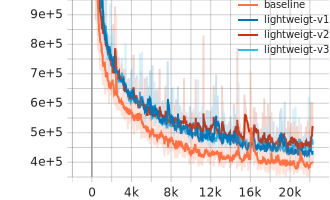
\includegraphics[width=\textwidth]{../history/loss_train_total.png}
        \caption{Training Loss}
    \end{subfigure}
    \hfill
    \begin{subfigure}[b]{0.4\textwidth}
        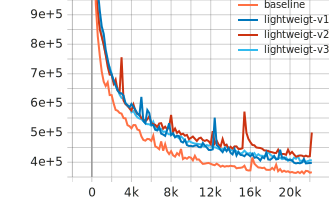
\includegraphics[width=\textwidth]{../history/loss_val_total.png}
        \caption{Validation Loss}
    \end{subfigure}
    \caption{Loss curves showing consistent convergence for all models.}
    \label{fig:loss}
\end{figure}

We also tracked the learning rate (Figure \ref{fig:lr}). The \texttt{ReduceLROnPlateau} scheduler reduced the learning rate when the validation loss plateaued, allowing for fine-grained optimization in later epochs.

\begin{figure}[h]
    \centering
    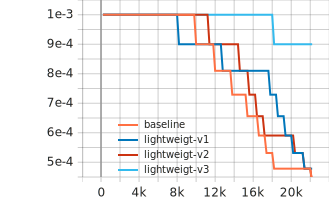
\includegraphics[width=0.4\textwidth]{../history/train_learning_rate.png}
    \caption{Learning Rate Schedule}
    \label{fig:lr}
\end{figure}

\subsection{Qualitative Analysis: Visual Quality}
We compared the output images generated by the models on the validation set and test set.

\textbf{Early Training (Step 800):} As observed in Table \ref{tab:validation}, the Baseline model learned the style features much faster than the lightweight variants. 
At step 800, the Baseline output is already easy to recognize, while the outputs of v1, v2, and v3 still look somewhat blurry.
This confirms that the lightweight models have a "Capacity Gap" and converge slower.


\begin{table}[htbp]
\centering
\setlength{\tabcolsep}{1pt}
\renewcommand{\arraystretch}{1} 
\begin{tabular}{ >{\raggedleft\arraybackslash}m{35pt} >{\centering\arraybackslash}m{3cm} >{\centering\arraybackslash}m{3cm} >{\centering\arraybackslash}m{3cm} >{\centering\arraybackslash}m{3cm} }
    
    % --- 表头行 ---
    & {\centering original} & {\centering 800 step} & {\centering 4200 step} & {\centering 21800 step} \\ 
    \\[-10pt] 
    
    % --- Baseline 行 ---
    baseline & 
    \img{../history/fixed_val_image.png} & 
    \img{../history/800-baseline.png} & 
    \img{../history/4200-baseline.png} & 
    \img{../history/21800-baseline.png} \\ 
    
    % --- V1 行 ---
    v1 & 
    \img{../history/fixed_val_image.png} & 
    \img{../history/800-v1.png} & 
    \img{../history/4200-v1.png} & 
    \img{../history/21800-v1.png} \\ 
    
    % --- V2 行 ---
    v2 & 
    \img{../history/fixed_val_image.png} & 
    \img{../history/800-v2.png} & 
    \img{../history/4200-v2.png} & 
    \img{../history/21800-v2.png} \\ 
    
    % --- V3 行 ---
    v3 & 
    \img{../history/fixed_val_image.png} & 
    \img{../history/800-v3.png} & 
    \img{../history/4200-v3.png} & 
    \img{../history/21800-v3.png} \\ 
\end{tabular}

\vspace{5pt} 
\caption{Comparison of a validation image at different training steps.}
\label{tab:validation}
\end{table}

\textbf{Final Result:} Despite the slower start, all models converged successfully by the end of training. 
Last columns (Step 4200 and Step 21800) of Table \ref{tab:validation} shows that althougth the loss curves continued to decrease, the visual quality improvements became less noticeable.
Table \ref{tab:tests_results} shows the final outputs on several test images.
Visually, the lightweight models (v1, v2, v3) are almost indistinguishable from the baseline in terms of global structure and color. 
The residual bottleneck appears to be highly redundant, as removing it caused little to no visual degradation.

\begin{table}[htbp]
\centering
\setlength{\tabcolsep}{1pt} 
\renewcommand{\arraystretch}{1} 
\begin{tabular}{ *{5}{ >{\centering\arraybackslash}m{3cm} } }
    
    original & baseline & lightweight-v1 & lightweight-v2 & lightweight-v3 \\ 
    \\[-10pt] % 增加一点垂直间距
    
    % 测试图片000000098497
    \img{../history/000000098497.jpg} & 
    \img{../history/000000098497_Baseline.jpg} & 
    \img{../history/000000098497_v1.jpg} & 
    \img{../history/000000098497_v2.jpg} & 
    \img{../history/000000098497_v3.jpg} \\ 

    % 测试图片000000545730
    \img{../history/000000545730.jpg} &
    \img{../history/000000545730_Baseline.jpg} &
    \img{../history/000000545730_v1.jpg} &
    \img{../history/000000545730_v2.jpg} &
    \img{../history/000000545730_v3.jpg} \\

    % 测试图片000000128598
    \img{../history/000000128598.jpg} &
    \img{../history/000000128598_Baseline.jpg} &
    \img{../history/000000128598_v1.jpg} &
    \img{../history/000000128598_v2.jpg} &
    \img{../history/000000128598_v3.jpg} \\
    
\end{tabular}

\vspace{5pt} 
\caption{Comparison of final stylized outputs on test images.}
\label{tab:tests_results}
\end{table}

\subsection{Specific Artifacts}
A specific artifact was observed in the lightweight models: 
checkerboard-distributed red spots appeared within the yellow celestial orbs (See the parts in Table \ref{tab:tests_results} that are marked with green squares.), 
which were less frequent in the baseline. 
This reduces the subjective quality slightly in high-contrast regions.



\section{Discussion}
\textbf{Capacity Gap and Convergence:} The lightweight models shows a slower convergence rate compared to the baseline. 
This is attributed to their reduced parameter capacity. 
However, the consistent decrease in both training and validation losses indicates that the lightweight architectures were successfully learning the style transfer task without suffering from overfitting.

\textbf{Artifacts from Decoupling:} We hypothesize that the "red spot" artifacts are a side effect of Depthwise Separable Convolutions. 
By decoupling spatial and channel-wise correlations, the network's ability to smooth out high-frequency color transitions locally might be reduced, leading to checkerboard-like patterns in specific style features.

\textbf{The Efficiency Trade-off:} While the lightweight variants introduced minor visual artifacts, they offered a compelling trade-off for deployment. 
The visual quality stopped improving after a few epochs of training, so twenty epochs were enough and training longer did not help much.

\section{Conclusion}
We successfully demonstrated that replacing standard convolutions with depthwise separable convolutions is a highly effective strategy for Neural Style Transfer. 
Our \textbf{Lightweight-v3} model offers a practical solution for deployment, achieving an \textbf{87\% size reduction} and \textbf{1.44x faster inference} with minimal impact on visual fidelity. 
Future work can include making the model smaller with methods such as quantization, and it can also include trying to remove red spots artifacts.

\bibliographystyle{unsrtnat}
\bibliography{references}

\end{document}